\documentclass[10pt,journal,cspaper,compsoc]{IEEEtran}
%
% If IEEEtran.cls has not been installed into the LaTeX system files,
% manually specify the path to it like:
% \documentclass[12pt,journal,compsoc]{../sty/IEEEtran}

\usepackage{fixltx2e}
% \usepackage{stfloats}
\usepackage{amsmath}
\usepackage{graphicx}
\usepackage{amsfonts}
\usepackage{amsthm}
\usepackage{cite}
\usepackage{algorithm}
\usepackage{algorithmic}
\usepackage{url}
\usepackage{caption}
\input{/Users/jovo/Research/latex/latex_commands.tex}
\hyphenation{op-tical net-works semi-conduc-tor}
\newcommand{\Qs}{Q}
% \newcommand{\mcL}{\mc{L}}
\newcommand{\mcS}{\mc{S}}
\newcommand{\mcU}{\mc{U}}


\begin{document}

\title{Shuffled Graph Classification:\\ Theory and Connectome Applications}

\author{Joshua T.~Vogelstein %, Mark Dredze, R.~Jacob~Vogelstein, 
 and 
Carey~E.~Priebe% <-this % stops a space
\IEEEcompsocitemizethanks{\IEEEcompsocthanksitem J.T. Vogelstein and C.E. Priebe are with the Department
of Applied Mathematics and Statistics, Johns Hopkins University, Baltimore, MD 21218.  %\protect\\
% note need leading \protect in front of \\ to get a newline within \thanks as
% \\ is fragile and will error, could use \hfil\break instead.
E-mail: \{joshuav,cep\}@jhu.edu
% \IEEEcompsocthanksitem R.J. Vogelstein is with the Johns Hopkins University Applied Physics Laboratory, Laurel, MD, 20723.
}% <-this % stops a space
\thanks{This work is partially supported by the Research Program in Applied Neuroscience.  The authors would like to thank Damianos Karakos for his helpful comments.}}
 
% The paper headers
\markboth{IN PREP}%
{Shuffled Graph Classification}

\IEEEcompsoctitleabstractindextext{%
\begin{abstract}
In this work, we investigate the extent to which shuffling vertex labels can hinder classification performance, and for which random graph models one might expect this shuffling to be impactful.  Via theory we demonstrate a collection of results.  Specifically, if one ``shuffles'' the graphs prior to classification, the vertex label information is irretrievably lost, which can degrade classification performance (and often does).  A specific graph-invariant classifier is shown to be Bayes optimal.  Moreover, this classifier may be induced by training data in a consistent and efficient fashion.  Unfortunately, both computational and sample size burdens make this ``plugin'' classifier impractical.  A graph-matched Frobenius norm $k_s$ nearest neighbor classifier, however, is also universally consistent as $s$ (the number of training samples) goes to infinity, and expected to converge faster whenever ``nearness'' implies same class.  Finally, we apply this approach to a connectome classification problem (a connectome is brain-graph where vertices correspond to (collections of) neurons and edges correspond to connections between them).  The graph-matched $k_s$NN classifier on the shuffled graphs performs better than a typical graph-invariant based $k_s$NN strategy, but not quite as well as the $k_s$NN on the labeled graphs, on a real connectome classification problem.  Thus, we demonstrate the practical utility of the theoretical derivations herein.  Extending these results to weighted and (certain) attributed random graph models is straightforward.  
\end{abstract}

% Note that keywords are not normally used for peer review papers.
\begin{keywords}
statistical inference, graph theory, network theory, structural pattern recognition, connectome.
\end{keywords}}


% make the title area
\maketitle
\IEEEdisplaynotcompsoctitleabstractindextext
\IEEEpeerreviewmaketitle



\section{Introduction} \label{sec:1}

\IEEEPARstart{R}{epresenting} data as graphs is becoming increasingly popular, as technological progress facilitates measuring ``connectedness'' in a variety of domains, including social networks, trade-alliance networks, and brain networks.  While the theory of pattern recognition is deep \cite{Devroye1996}, previous theoretical efforts regarding pattern recognition almost invariably assumed data are collections of vectors.  Here, we assume data are collections of graphs (where each graph is a set of vertices and a set of edges connecting the vertices).  For some data sets, the vertices of the graphs are \emph{labeled}, that is, one can identify the vertex of one graph with a vertex of the others.  For others, the labels are unobserved and/or assumed to not exist.  We investigate the theoretical and practical implications of the absence of vertex labels.  

These implications are especially important in the emerging field of ``connectomics'', the study of connections of the brain \cite{Hagmann05, Sporns2010}.  In connectomics, one represents the brain as a graph (a brain-graph), where vertices correspond to (groups of) neurons and edges correspond to connections between them.  In the lower part of the evolutionary hierarchy (e.g., worms and flies), many neurons have been assigned labels \cite{WhiteBrenner86}.  However, for even the simplest vertebrates, vertex labels are mostly unavailable when vertices correspond to neurons.  

Classification of brain-graphs is poised to become increasingly popular.  Although previous work has demonstrated some possible strategies of graph classification in both the labeled \cite{VP11_sigsub} and unlabeled \cite{Duin2011} scenarios, relatively little work has compared the theoretical limitations of the two.  We therefore develop a random graph model amenable to such theoretical investigations.  The theoretical results lead to practical universally consistent graph classification algorithms.  We demonstrate that these algorithms have desirable finite sample properties via a real brain-graph classification problem of significant scientific interest: sex classification.



% A common strategy for dealing with this ``unmatchedness'' is to operate in a quotient space of graphs.  In the quotient space, a vertex represents a collection of neurons, and this collection is assigned a label.  Edges become multi-edges, although they are commonly binarized to obtain simple graphs \cite{Hagmann2010}.  Operating in the quotient space of labeled vertices eases graph comparison, as the ``graph-matching'' sticky-wicket is avoided. Embedding the unlabeled graphs in this quotient space will likely be advantageous for some exploitation tasks, and disastrous for others (for instance, whenever the vertex labels contain all the signal for the specified task).  We aim to understand under what circumstances one could expect a classification performance degradation, and to what extent we can recover from losing the vertex label information.


% \IEEEPARstart{T}{his} work addresses graph classification in the presence of vertex label shuffling.   
% Consider the following idealized scenario.  Vertex labels may or may not be observed.  In the latter case, vertex $v$ in one graph cannot be assumed to correspond to vertex $v$ in another graph.  Comparing collections of graphs is therefore more difficult in this latent label situation. 


% Graph classification differs from classification of vector-valued random variables in several key aspects.  First, the structure of a graph may encode information.  Second, the vertex labels may or may not be observed.  In unobserved scenarios, NP-hard problems rear their ugly heads \cite{Conte2004}. 


\section{Graph Classification Models} % (fold)
\label{sec:shuffler_graph_class_models}

\subsection{A labeled graph classification model} % (fold)
\label{sub:a_labeled_graph_classification_model}

% subsection a_labeled_graph_classification_model (end)


A labeled graph $G=(\mc{V},\mc{E})$ consists of a vertex set $\mc{V}$, where $|\mc{V}|=n < \infty$ is the number of vertices, and an edge set $\mc{E}$, where $|\mc{E}| \leq n^2$.
\begin{defi}
Let $\GG\colon \Omega \to \mc{G}_n$ be a \emph{labeled} graph-valued random variable taking values $G\in \mc{G}_n$, where $\mc{G}_n$ is the set of labeled graphs on $n$ vertices.	
\end{defi}
The cardinality of $\mc{G}_n$ is super-exponential in $n$.  For example, when all labeled graphs are assumed to be simple (that is, undirected binary edges without loops), then $|\mc{G}_n|=2^{\binom{n}{2}}=d_n$. 
Let $Y$ be a categorical random variable, $Y\colon \Omega \to \mc{Y}=\{y_0,\ldots, y_{c}\}$, where $c< \infty$.  Assume the existence of a joint distribution, $\PP_{\GG,Y}$ which can be decomposed into the product of a class-conditional distribution (likelihood) $\PP_{\GG|Y}$ and a class prior $\pi_Y$. Because $n$ is finite, the class-conditional  distributions $\PP_{\GG | Y=y}=\PP_{\GG|y}$ can be considered discrete distributions $\text{Discrete}(G; \theta_y)$, where $\theta_y$ is an element of the $d_n$-dimensional unit simplex $\triangle_{d_n}$ (satisfying $\theta_{G|y}\geq 0$ $\forall G \in \mc{G}_n$ and $\sum_{G \in \mc{G}_n} \theta_{G|y}=1$).


% $\theta_y=[\theta_{1|y},\ldots \theta_{d|y}]\T \in \triangle_d$, where  $d=d_n=2^{\binom{n}{2}}$ and $\triangle_d$ is the $d$-dimensional simplex (that is, $\theta_{i|y}\geq 0$ for all $i \in [d]$ and $\sum_{i \in [d]} \theta_{i|y}=1$). 

\subsection{A shuffled graph classification model} % (fold)
\label{sub:a_shuffled_graph_classification_model}

% subsection a_shuffled_graph_classification_model (end)

% A shuffled graph $G'=(G,Q)$ consists of a labeled graph and a shuffling (vertex permutation) function $Q: \mc{G}_n \to \mc{G}_n$.  Let $\GG' \colon \Omega \to \mc{G}_n'$ be a shuffled graph-valued random variable taking values $G' \in \mc{G}_n'$, where $\mc{G}_n'$ is the set of shuffled graphs on $n$ vertices.  Moreover, let $\QQ$ be a permutation-valued random variable, $\QQ\colon\Omega \to \mc{Q}_n$, where $\mc{Q}_n$ is the space of vertex permutation functions on $n$ vertices so that $|\mc{Q}_n|=n!$. The cardinality of $\mc{G}_n'$ is therefore $|\mc{G}_n| n!$.  Note however, that $\QQ$ is a permutation of the vertices, thus realizations of $\QQ(\GG)$ must live within a set of cardinality $|\mc{G}_n|$.

% OLD PARAGRAPH BEGINS:
In the above, it was implicitly assumed that the vertex labels were observed.  However, in certain situations (such as the motivating connectomics example presented in Section \ref{sec:1}), this assumption is unwarranted.  To proceed, we define two graphs $G,G' \in \mc{G}_n$ to be isomorphic if and only if there exists a vertex permutation (shuffle) function $\Qs\colon\mc{G}_n \to \mc{G}_n$ such that $\Qs(G)=G'$.  Let $\QQ$ be a permutation-valued random variable, $\QQ\colon \Omega \to \mc{Q}_n$, where $\mc{Q}_n$ is the space of vertex permutation functions on $n$ vertices so that $|\mc{Q}_n|=n!$.  
% OLD PARAGRAPH ENDS
\begin{defi} \label{def:shuffled}
Let $\GG'=\QQ(\GG): \Omega \to \mc{G}_n$ be a \emph{shuffled} graph-valued random variable, that is, a labeled graph valued random variable that has been passed through a random shuffle channel $\QQ$. %Note that $|\mc{G}_n'|=|\mc{G}_n|$. % taking values $G\in \mc{G}_n$, where $\mc{G}_n$ is the set of labeled graphs on $n$ vertices.	
\end{defi}

Extending the above graph-classification model to include this vertex shuffling distribution yields $\PP_{\QQ,\GG,Y}$.  We assume throughout this work (with loss of generality) that the shuffling distribution is both \emph{class independent} and \emph{graph independent}; therefore, this joint model can be decomposed as
\begin{align}
	\PP_{\QQ,\GG,Y} = \PP_{\QQ} \PP_{\GG,Y} = \PP_{\QQ} \PP_{\GG |Y} \pi_Y = \PP_{\QQ(\GG) |Y} \pi_Y.
\end{align}
As in the labeled case, the shuffled graph class-conditional distributions $\PP_{\QQ(\GG)|y}$ can be represented by discrete distributions $\text{Discrete}(G; \theta_y')$.  Because $\QQ(\GG)$ can be any of $|\mc{G}_n|$ different graphs, it must be that $\theta_y' \in \triangle_{d_n}$.  When $\PP_{\QQ}$ is uniform on $\mc{Q}_n$, all shuffled graphs within the same isomorphism set are equally likely; that is  $\{\theta_{G_i|y}' = \theta_{G_j|y}' \, \forall G_i,G_j \colon \Qs(G_i)=G_j$ for some $\Qs \in \mc{Q}_n\}$.

Note that one can think of a labeled graph as a shuffled graph for which $\QQ$ is a point mass at  $Q=I$, where $I$ is the identity matrix.


\subsection{An unlabeled graph classification model} % (fold)
\label{sub:an_unlabeled_graph_classification_model}

% subsection an_unlabeled_graph_classification_model (end)

Let $\mt{\mc{G}}_n$ be the collection of isomorphism sets.
An \emph{unlabeled graph} $\mt{G}$ is an element of $\mt{\mc{G}}_n$. The number of unlabeled graphs on $n$ vertices is $|\mt{\mc{G}}_n|=\mt{d}_n \approx d_n/n!$ (see \cite{A000088} and references therein).
% , and $|\mt{\mc{G}}_n|=\mt{d}_n$.  
An \emph{unlabeling function} $U\colon \mc{G}_n \to \mt{\mc{G}}_n$ is a function that takes as input a graph and outputs the corresponding unlabeled graph. 
\begin{defi}
Let $\mt{\GG}=U(\GG)\colon \Omega \to \mt{\mc{G}}_n$ be an \emph{unlabeled} graph-valued random variable, that is, a labeled graph-valued random variable that has been passed through an unlabeled channel. In other words, $\mt{\GG}=\{Q(\GG)\}_{Q \in \mc{Q}_n}$, and takes values $\mt{G} \in \mt{\mc{G}}_n$. %$\colon \Omega \to \mt{\mc{G}}_n$ be an
\end{defi}  
The joint distribution over unlabeled graphs and classes is therefore
$\PP_{\mt{\GG},Y}=\PP_{U(\GG),Y}=\PP_{U(\QQ(\GG)),Y}$, which decomposes as $\PP_{\mt{\GG}|Y} \pi_Y$. The class-conditional distributions $\PP_{\mt{\GG} | y}$ over isomorphism sets (unlabeled graphs) can also be thought of as discrete distributions $\text{Discrete}(\mt{G}; \mb{\mt{\theta}}_y)$ where $\mb{\mt{\theta}}_y\in \triangle_{\mt{d}_n}$ are vectors in the $\mt{d}_n$-dimensional unit simplex.   Comparing shuffling and unlabeling for the independent and uniform shuffle distribution $\PP_{\QQ}$, we have $\{\theta_{G|y}'=\mt{\theta}_{\mt{G}|y}/|\mt{G}|$ for all $G \in \mt{G}\}$.  




\section{Bayes Optimal Graph Classifiers} % (fold)
\label{sec:bayes_optimal_graph_classifiers}

We consider graph classification in the three scenarios described above: labeled, shuffled, and unlabeled.  To proceed, in each scenario we define three mathematical objects: (i) a classifier, (ii) the Bayes optimal classifier, and (iii) the Bayes risk.

\subsection{Bayes Optimal Labeled Graph Classifiers} % (fold)
\label{sub:labeled_graph_classifiers}

% subsection labeled_graph_classifiers (end)

% \begin{itemize}
	% \item 
	A \emph{labeled graph classifier} $h\colon \mc{G}_n \to \mc{Y}$ is any function that maps from labeled graph space to class space. The risk of a labeled graph classifier $h$ under $0-1$ loss is the expected misclassification rate $L(h)=\EE[h(\GG)\neq Y]$, where the expectation is taken against $\PP_{\GG,Y}$.
	% \item  
	
	The \emph{labeled graph Bayes optimal classifier} is given by
	\begin{align}
		h_* = \argmin_{h \in \mc{H}} L(h),
	\end{align}
	where $\mc{H}$ is the set of possible labeled graph classifiers.
	% \item 
	
	The \emph{labeled graph Bayes risk} is given by 
	\begin{align}
		L_* =\min_{h \in \mc{H}} L(h),
	\end{align}
	where $L_*$ implicitly depends on $\PP_{\GG,Y}$.
% \end{itemize}



% A \emph{labeled} graph classifier $h\colon \mc{G}_n \to \mc{Y}$ is any function that maps from graph space to class space.  The \emph{risk} of a classifier under $0-1$ loss is the expected misclassification rate $L(h)=\EE[h(\GG)\neq Y]$, where the expectation is taken against $\PP_{\GG,Y}$.  
% \defa
% The \emph{labeled Bayes optimal graph classifier} $h_*$
% and \emph{labeled Bayes risk} $L_*=L(h_*)$
% are given by
% \begin{align}
% 	h_* &= \argmin_{h \in \mc{H}} L(h), \qquad %\\
% 	L_* =\min_{h \in \mc{H}} L(h),
% \end{align}
% where where $\mc{H}$ is the set of possible graph classifiers
% and $L_*$ implicitly depends on $\PP_{\GG,Y}$.  
% \defb
% The optimal classifier is the classifier that minimizes risk, also called the Bayes optimal graph classifier, given by
% \begin{align}
% 	h_* = \argmin_{h \in \mc{H}} L(h),
% \end{align}
% where $\mc{H}$ is the set of possible classifiers.  The  (which achieves the minimal (optimal) risk)  depends on $\PP_{\GG,Y}$.  

\subsection{Bayes Optimal Shuffled Graph Classifiers} % (fold)

A \emph{shuffled graph classifier} is also any function $h\colon \mc{G}_n \to \mc{Y}$ (note that the set of shuffled graphs is the same as the set of labeled graphs). However, by virtue of the input being a shuffled graph as opposed to a labeled graph, the shuffled risk under $0-1$ loss is given by $L'(h)=\EE[h(\QQ(\GG)) \neq Y]$, where the expectation is taken against $\PP_{\QQ(\GG),Y}$. %As above, 
% \begin{align}
% h'_*=\argmin_{h \in \mc{H}} L'(h).	
% \end{align}
% The \emph{shuffled Bayes risk}, $L'_*=L'(h'_*)$, depends on $\PP_{\QQ,\GG,Y}$.
% \defa

The \emph{shuffled graph Bayes optimal classifier} is given by
\begin{align}
	h_*' &= \argmin_{h \in \mc{H}} L'(h), %, \qquad %\\
\end{align}
where $\mc{H}$ is again the set of possible labeled (or shuffled) graph classifiers. The \emph{shuffled graph Bayes risk} is given by
\begin{align}
	% h_*' &= \argmin_{h \in \mc{H}} L'(h), \qquad %\\
	L_*' =\min_{h \in \mc{H}} L'(h),
\end{align}
where  $L_*'$ implicitly depends on $\PP_{\QQ(\GG),Y}$.  % \defb

\subsection{Bayes Optimal Unlabeled Graph Classifiers} % (fold)


An \emph{unlabeled} graph classifier $\mt{h}\colon \mt{\mc{G}}_n \to \mc{Y}$ is any function that maps from unlabeled graph space to class space. The risk under $0-1$ loss is given by $\mt{L}(\mt{h})=\EE[\mt{h}(\mt{\GG})\neq Y]$, where the expectation is taken against $\PP_{\mt{\GG},Y}$. 

% \defa
The \emph{unlabeled graph Bayes optimal classifier} is given by %$\mt{h}_*$
\begin{align}
	\mt{h}_* &= \argmin_{\mt{h} \in \mt{\mc{H}}} L(\mt{h}), \qquad %\\
	% \mt{L}_* =\min_{\mt{h} \in \mt{\mc{H}}} L(\mt{h}),
\end{align}


% where $\mt{L}_*$ implicitly depends on $\PP_{\mt{\GG},Y}$.  

The \emph{unlabeled graph Bayes risk} is given by %$\mt{L}_*=L(\mt{h}_*)$
% are given by
\begin{align}
	% \mt{h}_* &= \argmin_{\mt{h} \in \mt{\mc{H}}} L(\mt{h}), \qquad %\\
	\mt{L}_* =\min_{\mt{h} \in \mt{\mc{H}}} L(\mt{h}),
\end{align}
where $\mt{\mc{H}}$ is the set of possible unlabeled graph classifiers
and $\mt{L}_*$ implicitly depends on $\PP_{\mt{\GG},Y}$.  
% \defb

% The Bayes optimal unlabeled graph classifier is given by
% \begin{align}
% 	\mt{h}_*=\argmin_{\mt{h} \in \mt{\mc{H}}} \mt{L}(\mt{h}).
% \end{align}
% The \emph{unlabeled Bayes risk},  $\mt{L}_*=\mt{L}(\mt{h}_*)$,  depends on $\PP_{\mt{\GG},Y}$.

\subsection{Parametric Classifiers} % (fold)
\label{sub:parametric_classifiers}

% subsection parametric_classifiers (end)

The three Bayes optimal graph classifiers can be written explicitly in terms of their model parameters:
\begin{align}
	h_*(G) &= \argmax_{y \in \mc{Y}} \theta_{G|y}\pi_y, \label{eq:La_Bayes} \\
	h_*'(G) &= \argmax_{y \in \mc{Y}} \theta_{G|y}' \pi_y,  \label{eq:Sh_Bayes} \\
	\mt{h}_*(\mt{G}) &= \argmax_{y \in \mc{Y}}  \mt{\theta}_{\mt{G}|y}\pi_y. \label{eq:Un_Bayes}
\end{align}


% section bayes_optimal_graph_classifiers (end)


\section{Theoretical Implications of Shuffling} % (fold)
\label{sec:theoretical_results}

% section theoretical_results (end)
\subsection{Shuffling Can Degrade Optimal Performance} % (fold)
\label{sec:shuffle}


% For brevity, we will use the shorthand $\PP_y=\PP_{\GG | Y = y}=\theta_{G|y}$, $\mt{\PP}_y=\PP_{\mt{\GG} | Y = y}=\mt{\theta}_{\mt{G}|y}$ and $\PP'_y=\PP_{\GG'|Y=y}'=\theta_{G'|y}'$. 



The result of either shuffling or unlabeling a graph can only degrade, but not improve Bayes risk.  This is a restatement of the data processing lemma for this scenario. Specifically, \cite{Devroye1996} shows that the data processing lemma indicates that in the classification domain $L^*_X \leq L^*_{T(X)}$ for any transformation $T$ and data $X$.  In our setting, this becomes:

\begin{thm} \label{thm:1}
$L_* \leq \mt{L}_*=L_*'$.
\end{thm}

\begin{proof}
	Assume for simplicity $|\mc{Y}|=2$ and $\pi_0=\pi_1=1/2$.  
\begin{align} \label{eq:thm1}
	\mt{L}_*&=\sum_{\mt{G} \in \mt{\mc{G}}_n} \min_y  \mt{\theta}_{\mt{G}|y}  
	=\sum_{\mt{G} \in \mt{\mc{G}}_n} \min_y  \sum_{G \in \mt{G}}\theta_{G|y}'  = L_*' \nonumber \\
	&=\sum_{\mt{G} \in \mt{\mc{G}}_n} \min_y  \sum_{G \in \mt{G}}\theta_{G|y} 
	 \geq \sum_{\mt{G} \in \mt{\mc{G}}_n} \sum_{G \in \mt{G}} \min_y  \theta_{G|y}  = L_*.
	% & \geq \sum_{\mt{G} \in \mt{\mc{G}}_n}\sum_{G' \in \mt{G}}\min_y\PP_y(G')=L_*.
\end{align}
% It is trivially true that $\mt{L}_*=L_*'$.
\end{proof}



An immediate consequence of the above proof is that the inequality in the statement of Theorem \ref{thm:1} strict whenever the inequality in Eq. \eqref{eq:thm1} is strict:

\begin{thm} \label{thm:2}
	$L_* < \mt{L}_*=L'_*$ if and only if there exists $\mt{G}$ such that
	% $$\min_y \mt{\PP}_{y}(\mt{G}) > \sum_{G' \in \mt{G}}\min_y\PP_y(G').$$
	$$\min_y \mt{\theta}_{\mt{G}|y} > \sum_{G \in \mt{G}}\min_y \theta_{G|y}.$$
\end{thm}
The above result demonstrates that even when the labels \emph{do} carry some class-conditional signal, it may be the case that shuffling or unlabeling does not degrade performance.  In other words, the following two statements are equivalent: (i) the labels contain information with regard to the classification task, and (ii) some graphs within an isomorphism set are class-conditionally more likely than others: $\exists \, \theta_{G_i|y} \neq \theta_{G_j|y}$ where $\Qs(G_i)=G_j$ for some $G_i,G_j \in \mc{G}_n$, $\Qs \in \mc{Q}_n$, and $y \in \mc{Y}$%, and that $\theta_{G_i|y}\neq \theta_{G_i|y'}$ or $\theta_{G_j|y}\neq \theta_{G_j|y'}$
.  Shuffling has the effect of ``flattening'' likelihoods within isomorphism sets, from $\theta_y$ to $\theta_y'$, so that $\theta_y'$ satisfies $\{\theta_{G|y}'=\mt{\theta}_{\mt{G}|y}/|\mt{G}| \, \forall \colon G \in \mt{G}\}$.  But just because the shuffling changes class-conditional likelihoods does \emph{not} mean that Bayes risk must also change. This result follows immediately upon realizing that posteriors can change without classification performance changing.  The above results are easily extended to consider non-equal class priors and $c$-class classification problems.  To see this, ignoring ties, simply replace each minimum likelihood with a sum over all non-maximum posteriors: 
% $$\min_y \PP_y(G) \to \sum_{y \in \mc{Y}'} \PP_y(G) \text{ where } \mc{Y}' =\{y : y \neq \argmax_y \PP_y\}.$$
\begin{multline}
\min_y \theta_{G|y} \pi_y \mapsto \sum_{y \in \mc{Y}'} \theta_{G|y} \pi_y \\ \text{ where } \mc{Y}' =\{y \colon y \neq \argmax_y \theta_{G|y}\}.
\end{multline}

\subsection{Bayes Optimal Graph Invariant Classification After Shuffling} % (fold)
\label{sec:gi}

A graph invariant on $\mc{G}_n$ is any function $\psi$  such that $\psi(G)=\psi(\Qs(G))$ for all $G \in \mc{G}_n$ and $\Qs \in \mc{Q}_n$.  A graph invariant classifier is a composition of a classifier with an invariant function, $h^\psi=f^\psi \circ \psi$.  The Bayes optimal graph invariant classifier minimizes risk over all invariants: 
\begin{align} \label{eq:psi}
	h_*^{\psi}=\argmin_{\psi \in \Psi, f^{\psi} \in \mc{F}^{\psi}} \EE[f(\psi(\GG))\neq Y],
\end{align}
where $\Psi$ is the space of all possible invariants and $\mc{F}^{\psi}$ is the space of classifiers composable with invariant $\psi$. The expectation in Eq. \eqref{eq:psi} is taken against $\PP_{\GG,Y}$ or equivalently $\PP_{\QQ(\GG),Y}$, since invariants are invariant.
  Let $L_*^{\psi}$ denote the Bayes invariant risk.  
\begin{thm} \label{thm:3}
	$\mt{L}_*=L_*^\psi$.
\end{thm}

\begin{proof}
Let $\psi$ indicate in which equivalence set $G$ resides; that is,  $\psi(G)=\mt{G}$ if and only if $G \in \mt{G}$.  Then
% $f_{G'}(G)$ be a graph matching function; that is, $f\colon \mc{G}_n \times \mc{G}_n \to \{0,1\}$, taking value unity whenever $G$ and $G'$ are isomorphic to one another.  Let $\psi(G)=\mb{f}(G)$, where $\mb{f}=(f_{G_1}, \ldots, f_{G_{\mt{d}}})$.  In words, $\phi(G)$ outputs a vector of length $\mt{d}_n$ with a single non-zero entry in the isomorphism set of $G$.  Let $h^{\psi}$ be an indicator function for the maximum a posteriori class of the corresponding isomorphism set. For instance, if $G \in \mt{G}_j$, then
\begin{align}
	h^{\psi}_*(G) &= \argmax_{y \in \mc{Y}} \mt{\theta}_{\psi(G)|y} \pi_y \nonumber \\
	&= \argmax_{y \in \mc{Y}} \mt{\theta}_{\mt{G}|y} \pi_y = \mt{h}_*(G).
\end{align}
% Thus, this graph invariant based classifier is the unlabeled Bayes optimal classifier.
\end{proof}



\section{Learning Optimal Classifiers from Data} % (fold)
\label{sec:learning_optimal_classifiers_from_data}

Section \ref{sec:shuffle} shows that one cannot fruitfully ``unshuffle'' graphs: once they have been shuffled by a uniform shuffler, any label information is lost.  Section \ref{sec:gi} shows that if graphs have been uniformly shuffled, there is a relatively straightforward algorithm for optimal classification. However, that classifier depends on knowing the parameters.
%, $\mt{\theta}=\{\mt{\theta}_y\}_{y\in \mc{Y}}$ and $\mb{\pi}=\{\pi_y\}_{y \in \mc{Y}}$. 
When the parameters are unknown (effectively always), we assume that the data are sampled identically and independently from some unknown joint distribution: $(\QQ_i(\GG_i),Y_i)\overset{iid}{\sim}\PP_{\QQ,\GG,Y}$.  
For \emph{labeled} graph classification, $\PP_{\QQ}$ is assumed to be the identity function, therefore, $\mc{T}_s=\{(\GG_i,Y_i)\}_{i \in [s]}$, because when graphs are labeled $\QQ_i(\GG_i)=\GG_i$.
% the training data are $\mc{T}_s=\{(\GG_i,Y_i)\}_{i \in [s]}$, where $[s]=\{1,\ldots,s\}$ (because $\QQ_i$ is assumed to be a known point mass).  
For \emph{shuffled} graph classification $\PP_{\QQ}$ is assumed to be uniform over the permutation matrices, so that all label information is both unavailable and irrecoverable.  The training data are therefore $\mc{T}_s'=\{(\GG_i',Y_i)\}_{i \in [s]}$, where $\GG_i'=\QQ_i(\GG_i)$.  For \emph{unlabeled} graph classification the training data are again $\mc{T}_s'$. 
%We assume that $\PP_{\QQ}$ is uniform, so that all label information is both unavailable and irrecoverable.  
Our task is to utilize training data to induce a classifier
% $\mh{h}_s\colon \mc{G}_n \times (\mc{G}_n \times \mc{Y})^s \to \mc{Y}$ 
that approximates 
% $\mt{h}_*$ 
a Bayes classifier
as closely as possible.  


% section learning_optimal_classifiers_from_data (end)

\subsection{Bayes Plug-in Graph Classifiers} %} % (fold)
\label{sec:bayes_optimal_graph_invariant_based_classifier}



A \emph{labeled} graph Bayes plugin classifier,
$\mh{h}_s: \mc{G}_n \times \{(\GG_i,Y_i)\}_{i \in [s]} \to \mc{Y}$,
estimates the parameters $\{\theta_y,\pi_y\}_{y \in \mc{Y}}$ using the training data $\mc{T}_s=\{(\GG_i,Y_i)\}_{i \in [s]}$, and then plugs those estimates into the labeled Bayes classifier, Eq. \eqref{eq:La_Bayes}, resulting in
\begin{align} \label{eq:La_Plug}
	\mh{h}_s(G)=\argmax_{y\in\mc{Y}} \hth_{G|y}\mh{\pi}_y.
\end{align}

A \emph{shuffled} graph Bayes plugin classifier,
$\mh{h}_s': \mc{G}_n \times \{(\GG_i',Y_i)\}_{i \in [s]} \to \mc{Y}$,
estimates the parameters $\{\theta_y',\pi_y\}_{y \in \mc{Y}}$ using the training data $\mc{T}_s'=\{(\GG_i',Y_i)\}_{i \in [s]}$, and then plugs those estimates into the shuffled Bayes classifier, Eq. \eqref{eq:Sh_Bayes}, resulting in
\begin{align} \label{eq:Sh_Plug}
	\mh{h}_s'(G)=\argmax_{y\in\mc{Y}} \hth_{G|y}'\mh{\pi}_y.
\end{align}

An \emph{unlabeled} graph Bayes plugin classifier,
$\mh{\mt{h}}_s: \mc{G}_n \times \mc{T}_s' \to \mc{Y}$,
first determines in which unlabeled set each shuffled graph resides, using $\psi$ as defined in Section \ref{sec:gi}.  Then, it estimates the parameters $\{\mt{\theta}_{\psi(G')|y}\}_{y \in \mc{Y}}$ and $\{\pi_y\}_{y \in \mc{Y}}$ using the training data $\mc{T}_s'$. Finally, it plugs those estimates into the unlabeled Bayes classifier, Eq. \eqref{eq:Un_Bayes}, resulting in
\begin{align} \label{eq:Sh_Plug}
	\mh{\mt{h}}_s(G)=\argmax_{y\in\mc{Y}} \mh{\mt{\theta}}_{\mt{G}|y}\mh{\pi}_y.
\end{align}

% An unlabeled graph Bayes \emph{plugin} classifier estimates the likelihood and prior terms and plugs them in to Eq. \eqref{eq:unbayes2}:
% \begin{align} \label{eq:Sh_Plug}
% 	\mh{h}_s(\mt{G})=\argmax_{y\in\mc{Y}} \mh{\mt{\theta}}_{\mt{G}|y}\mh{\pi}_y. %, \text{ where } G\in \mt{G}_j.
% \end{align}

For brevity, we will sometimes refer to the above three induced classifiers as simply ``classifiers''.  Moreover, the sequence of classifiers (for example, $\{h_s\}_{s \to \infty}$) we will also refer to as a ``classifier''. 

\subsubsection{The Existence and Uniqueness of Universally Consistent Bayes Plug-in Graph Classifiers} % (fold)
\label{sub:bayes_plug_in_classifiers_are_consistent}

% subsection bayes_plug_in_classifiers_are_consistent (end)


For the above three classifiers, there exist estimators such that the classifiers exist, are unique, and moreover, are universally consistent, although the relative convergence rates and values that they converge to differ.

Let $\mh{L}_s=L(\mh{h}_s)$ be the risk of the induced \emph{labeled} graph Bayes plugin classifier using the training data $\mc{T}_s$ to obtain maximum likelihood estimators for $\{\theta_y,\pi_y\}_{y \in \mc{Y}}$. Note that $\mh{L}_s$ is a random variable, as it is a function of the random training data $\mc{T}_s$. This yields
\begin{thm} \label{thm:4}
	$\mh{L}_s \pconv L_*$ as $s \conv \infty$.
\end{thm}
\begin{proof}
Because ${\mc{G}}_n$ and $\mc{Y}$ are both finite, the maximum likelihood estimates for the categorical parameters $\{\theta_y,\pi_y\}_{y \in \mc{Y}}$ are guaranteed to exist and be unique \cite{Devroye1996}.  Hence, the labeled graph Bayes plugin classifier is universally consistent to ${L}_*$ (that is, it converges to ${L}_*$ regardless of the true joint distribution, $\PP_{\QQ, \GG ,Y}$) \cite{Devroye1996}. 
% Note that this classifier is universally consistent, meaning that it converges to . %Formally, if $\mhb{\mt{\theta}} \conv \mb{\mt{\theta}}$ and $\mhb{\pi} \conv \mb{\pi}$ as $s \conv \infty$, then $\mh{L}_s \conv \mt{L}_*$ as $s\conv \infty$.  
% Thus, $\mh{h}_s \conv \mt{h}_*$ as $s \conv \infty$.
\end{proof}

Similarly, let $\mh{L}_s'=L(\mh{h}_s')$ be the risk of the induced \emph{shuffled} graph Bayes plugin classifier using the training data $\mc{T}_s'$ to obtain maximum likelihood estimators for $\{\theta_y',\pi_y\}_{y \in \mc{Y}}$.  This yields
\begin{coro} \label{cor:Sh_Plug}
	$\mh{L}_s' \pconv L_*'$ as $s \conv \infty$.
\end{coro}
\begin{proof}
	The above proof rests on the finitude of $\mc{G}_n$, which remains finite after shuffling (uniform or otherwise), and therefore, the above proof holds, replacing $L_*$ with $L_*'$.
\end{proof}


% one could simply take the shuffled graph data $\mc{T}_s'$, without using $\psi$ (as defined above), and estimate $\theta_y'$.  While silly (as we know that ), this procedure is still asymptotically optimal.  Let $\mh{L}_s'$ be the risk of the induced \emph{shuffled} graph Bayes plugin classifier obtaining maximum likelihood estimates from $\mc{T}_s'$ to obtain the plugin estimate for Eq. \eqref{eq:Sh_Plug}. As above,  it follows that

Thus while one could merely plug the shuffled graphs into $\theta_y'$, such a procedure is inadvisable.  Specifically, the above procedure does not  use the fact that all $\theta_{G_i'|y} = \theta_{G_j'|y}$ whenever $Q(G_i)=G_j$ for some $Q \in \mc{Q}$.  Instead, consider the risk $\mh{\mt{L}}_s=L(\mh{\mt{h}}_s)$ of the induced \emph{unlabeled} graph Bayes plugin classifier upon using the $\psi$ function to map each shuffled graph to its corresponding unlabeled graph, and then obtaining maximum likelihood estimates of the unlabeled graph parameters, $\mt{\theta}$.  
\begin{coro} \label{cor:Un_Plug}
	$\mh{\mt{L}}_s \pconv \mt{L}_*$ as $s \conv \infty$.
\end{coro}

Because $|\mt{\mc{G}}_n| \ll |\mc{G}_n|$ (by a factor of approximately $n!$), it follows that classifying by first projecting the graphs into a lower dimensional space should yield improved performance.  Specifically, we have the following result:
%% perhaps to uncomment
% although both $\mh{h}_s'$ and $\mh{\mt{h}}_s$ are universally consistent, $\mh{h}_s'$ will generally perform worse.  
% In fact, we have the following result:
% \begin{thm} \label{thm:inadmiss}
% 	$\mh{h}_s$ dominates $\mh{h}_s'$. 
% \end{thm}
% \begin{proof}
% 	To see that $\mh{h}_s'$ is inadmissible with respect to $\mh{h}_s$ under $0-1$ loss with expected misclassification risk, it is sufficient to show that the expected distance between  $\hth_s$ and $\theta$ is smaller than that of $\hth_s'$ and $\theta$, for all $s$. Note that while the training data for $\hth_s$ is $\mc{T}_s$, the training data for $\hth_s'$ is $\mc{T}_s'$. We formalize this as follows:
% 	\begin{subequations}
% 	\begin{align}
% 		\EE[\norm{\hth_s - \theta}_2^2] &\leq \EE[\norm{\hth_s - \theta}_2^2] \\
% 		\EE[{\hth_s}\T \hth_s - 2 \theta\T \hth_s - \theta\T \theta ] &\leq 	\EE[(\hth_s')\T \hth_s - 2 \theta\T {\hth_s}' - \theta\T \theta ] \\
% 		\VV[\hth_s] -2 \theta\T \EE[\hth_s] &\leq 	\VV[{\hth_s}'] -2 \theta\T \EE[{\hth_s}'] \\
% 		\VV[\hth_s] -2 \theta\T\theta &\leq 	\VV[{\hth_s}'] -2 \theta\T\theta',
% 	\end{align}
% \end{subequations}
% 	where $\VV[\cdot]$ indicates the variance operator. That the final inequality is true follows from the following two results.  First, $\theta\T \theta' \leq \theta\T \theta$ because the parameter vectors necessarily have the same magnitude.  Second, the variance of $\theta_s'$ is necessarily no smaller than the variance of $\theta_s$, because $\theta_s'$ operates on the same input as $\theta_s$ does, except that it has been shuffled.
% \end{proof}

\begin{thm} \label{thm:tdomp}
	$\mh{\mt{h}}_s$ dominates $\mh{h}_s'$. 	
\end{thm}
\begin{proof}
% $\EE[\mh{L}_s'] \geq \EE[\mh{\mt{L}}_s]$ for all $s$.
% 	The first inequality follows from $\hth'_{G|y}$ converging to $\theta'_{G|y}$ slower than $\mh{\mt{\theta}}_{\mt{G}|y}$ converges to $\mt{\theta}_{\mt{G}|y}$.  Although $\theta'_{G|y}$ and  $\mt{\theta}_{\mt{G}|y}$ encode identical information, the dimensionality of the two differs drastically.  Specifically, $\mt{\theta}_{\mt{G}|y} \in \triangle_{\mt{d}_n}$ and $\theta'_{\mt{G}|y} \in \triangle_{d_n}$, and $\mt{d}_n \approx d_n/n!$.
% The proof of this corollary is similar to the above proof, so we merely sketch it here.  
Because $\htth_s$ can borrow strength from all the shuffled graphs within an unlabeled graph, its variance is smaller than the variance of $\hth_s'$.  
% Moreover, if vertex labels are available, $\mh{\mt{h}}_s$ is also inadmissible under $0-1$ loss.  
\end{proof}

% \begin{proof}
% Because $\mt{\mc{G}}_n$ and $\mc{Y}$ are both finite, their respective maximum likelihood estimates are guaranteed consistent by the law of large numbers.  Hence,  the unlabeled graph Bayes plugin classifier is also consistent to $\mt{L}_*$ \cite{DEV96}. Note that this classifier is universally consistent, meaning that it converges to $\mt{L}_*$ regardless of the true joint distribution, $\PP_{\QQ(\GG) ,Y}$. %Formally, if $\mhb{\mt{\theta}} \conv \mb{\mt{\theta}}$ and $\mhb{\pi} \conv \mb{\pi}$ as $s \conv \infty$, then $\mh{L}_s \conv \mt{L}_*$ as $s\conv \infty$.  
% % Thus, $\mh{h}_s \conv \mt{h}_*$ as $s \conv \infty$.
% \end{proof}


% As described above, the class-conditional distributions of unlabeled graphs can be characterized as  categorical distributions, $\PP_{\mt{\GG}|Y=y}=\text{Cat}(\mb{\mt{\theta}}_y)$.  Because a categorical distribution is in the exponential family, the maximum likelihood estimate for its parameters are exist, are unique, consistent, and efficient.  Moreover, the class prior can also be represented as a categorical random-variable, and therefore has the same properties.  Taken together, these results demonstrate that the Bayes plugin unlabeled graph classifier is consistent and efficient.

\subsection{$k$ Nearest Neighbor Universally Consistent Graph Classifiers} % (fold)
\label{sec:a_practical_approach_to_unlabeled_graph_classification}


Corollary \ref{cor:Sh_Plug} demonstrates that one can induce a universally consistent classifier $\mh{\mt{h}}_s$  using Eq. \eqref{eq:Sh_Plug}. Theorem \ref{thm:tdomp} further shows that the performance of $\mh{\mt{h}}_s$ dominates $\mh{h}_s'$.  Yet, using $\mh{\mt{h}}_s$ is practically useless for two reasons.  First, it requires solving $s$ graph isomorphism problems. Unfortunately, there are no known algorithms for solving graph isomorphism problems with worst-case performance in only polynomial time \cite{Fortin1996}. Second, the number of parameters to estimate is super-exponential in $n$ ($\mt{d}_n \approx 2^{n^2}/n!$), and acceptable performance will typically require $s \gg \mt{d}_n$.  We can therefore not even store the parameter estimates for small graphs (e.g., $n=30$), much less estimate them.  
% Specifically, using Eq. \eqref{eq:Sh_Plug} requires first enumerating  all $\mt{d}_n$ isomorphism sets, then determining in which isomorphism set the to-be-classified graph and each of the training graphs reside.  This approach is therefore, in general, impractical because the number of parameters to estimate, $\mt{d}_n$, is too large. 
This motivates consideration of an alternative strategy.

A $k_s$ nearest-neighbor classifier 
using Euclidean norm distance
is universally consistent to $L_*$ for vector-valued data 
% labeled graph classification 
as long as $k_s \conv \infty$ with $k_s/s \conv 0$ as $s \conv \infty$ \cite{Stone1977}. This non-parametric approach circumvents the need to estimate many parameters in high-dimensional settings such as graph-classification. The universal consistency proof for $k_s$NN was extended to graph-valued data in \cite{VP11_super}, which we include here for completeness.   Specifically, to compare labeled graphs, \cite{VP11_super} considered a Frobenius norm distance
\begin{align}
	\delta(G_i,G_j)=\norm{A_i-A_j}_F^2,
\end{align}
where $A_i$ is the adjacency matrix representation of the labeled graph, $G_i$.  
Let $\mh{h}_s^\delta$ denote the Frobenius norm $k_s$NN classifier on \emph{labeled} graphs using $\delta$, and let $\mh{L}^{\delta}_s$ indicate the misclassification rate for this classifier.  \cite{VP11_super} showed:
\begin{thm} \label{thm:5}
	$\mh{L}^{\delta}_s \pconv L_*$ as $s \conv \infty$.
\end{thm}
\begin{proof}
Because both $\mc{G}$ and $\mc{Y}$ have finite cardinality, the law of large numbers ensures that eventually as $s \conv \infty$, the plurality of nearest neighbors to a test graph will be identical to the test graph. 
\end{proof}
Let ${\mh{h}}^{'\delta}_s$ indicate the Frobenius-norm $k_s$NN on \emph{shuffled} graphs using $\delta$, and let $\mh{L}^{'\delta}_s$ indicate the misclassification rate for this classifier.  %Similarly, let ${\mh\mt{h}}^{\delta}_s$ and $\mh{\mt{L}}^{\delta}_s$ be the Frobenius-norm $k_s$NN on \emph{unlabeled} graphs using
From above theorem, the fact that $|\mc{G}_n'|=|\mc{G}_n|$ (see Definition \ref{def:shuffled}), and Corollary \ref{cor:Sh_Plug},  the below follows immediately:
\begin{coro} \label{cor:knn1}
	$\mh{L}^{'\delta}_s \pconv L_*'$ as $s \conv \infty$.
\end{coro}

Given shuffled graph data $\mc{T}_s'$, however, other distance metrics appear more ``natural'' to us.  For example,  
% As mentioned above, the number of unlabeled graphs is vastly less than the number of labeled or shuffled graphs, $|\mt{\mc{G}}_n| \approx |\mc{G}_n|/n!$.  Therefore, given that we observed only labeled or shuffled graphs, but not unlabeled graphs, we 
consider the ``graph-matched Frobenius norm'' distance:
\begin{align} \label{eq:d}
\delta'(G_i',G_j')=\min_{Q \in \mc{Q}_n}\norm{Q(A_i')-A_j'}_F^2,	
\end{align}
where $A_i'$ and $A_j'$ are shuffled adjacency matrices.  
Let $\mh{h}^{'\delta'}_s$ indicate the misclassification rate of the $k_s$NN classifier using the above graph-matched norm $\delta'$ \emph{shuffled} graphs, and let $\mh{L}^{'\delta'}_s$ indicate the misclassification rate for this classifier.  Given an exact graph matching function---a function that actually solves Eq. \eqref{eq:d}---we have the following result:
% we can use this as the distance in a $k_s$NN algorithm, referred to as the GM-$k_s$NN. 
% The GM-$k_s$NN classifier for shuffled graphs proceeds as follows.  First, compute the graph-matched Frobenius norm distance between the test graph $G$ and all training graphs, $\{\delta_i=\delta(G,G_i)\}_{i \in [s]}$.  Second, order the graph/class pairs according to their distances, $\delta_{(1)} \leq \cdots \leq \delta_{(s)}$.  Finally, let the estimated class be the plurality class of the $k_s$ closest graphs; that is, $\mh{y}=\argmax_{y \in \mc{Y}} \sum_{i \in [k_s]} \II\{y_{(i)}=y\}$.   %Collectively, we refer to this classification strategy as \emph{graph-matched} $k_s$NN (GM-$k_s$NN).
\begin{coro} \label{cor:Sh_knn}
	$\mh{L}^{'\delta'}_s \pconv L_*'$ as $s \conv \infty$.
\end{coro}
Thus, given shuffled data $\mc{T}_s'$, one could consider either $\mh{h}_s^{\delta}$ or $\mh{h}_s^{'\delta'}$.  Analogous to the Bayes plugin results above, for the $k_s$NN classifiers, we have 
\begin{thm} \label{thm:knninadmiss}
	$\mh{h}_s^{'\delta'}$ dominates $\mh{h}_s^{\delta}$ when data are \emph{shuffled} graphs.
	% $\EE[\mh{L}^{\delta'}_s] \geq \EE[\mh{L}^{\mt{\delta}}_s], \EE[\mh{L}^{\delta}_s]$ for all $s$. 
\end{thm}
\begin{proof}
	% The graph-matched classifier, $\mh{h}_s^{\mt{\delta}}$, however, borrows strength from all training shuffled graphs within the same isomorphism set as a test shuffled graph, whereas $\mh{h}_s^{\delta'}$ does not.  
	The above domination follows from the following consideration:  
	% Both $\mh{h}_s^{\delta}$ and $\mh{h}_s^{'\delta'}$ operate on $\mc{T}_s'$.  
	$\mh{h}_s^{\delta'}$ only benefits from graphs that have been shuffled identically, whereas $\mh{h}_s^{'\delta'}$  benefits from all graphs within an equivalence class, regardless of how they have been shuffled. Therefore, $\mh{h}^{\delta}_s$ is inadmissible with respect to $\mh{h}_s^{'\delta'}$ under the expected risk of $0-1$ loss. \end{proof}
% 	Moreover, if vertex label information is available, $\mh{h}^{\delta}_s$ is also inadmissible under $0-1$ loss.

Interestingly, when the data are labeled graphs, $\mc{T}_s$, one can outperform $\mh{h}_s^{\delta}$ by \emph{shuffling}, that is, by apparently destroying the label information.  Consider an example in which $\theta=\theta'$, such that no information is in the labels.  In such scenarios, shuffling can effectively borrow strength from different labeled graphs that are within the same unlabeled graph set. Let $\mh{h}^{\delta'}_s$ indicate the misclassification rate of the $k_s$NN classifier using $\delta'$ \emph{labeled} graphs, and let $\mh{L}^{\delta'}_s$ indicate the misclassification rate for this classifier. We therefore state without proof:
\begin{thm} \label{thm:nodom}
	Neither $\mh{h}_s^{\delta'}$ nor $\mh{h}_s^{\delta}$ dominates when data are \emph{labeled} graphs.
	% $\EE[\mh{L}^{\delta'}_s] \geq \EE[\mh{L}^{\mt{\delta}}_s], \EE[\mh{L}^{\delta}_s]$ for all $s$. 
\end{thm}



Thus, when the training data consists of shuffled graphs, the best universally consistent classifier (of those considered herein) is a $k_s$NN that uses $\delta'$ as the distance metric.  Other universally consistent classifiers that we considered either require estimating more parameters than there are molecules in the universe, or are inadmissible under $0-1$ loss.  When vertex labels are available, no classifier dominates. 


\subsection{Other Graph Invariants are Worse} % (fold)
\label{sub:asymptotically_optimal_classifiers}

% subsection asymptotically_optimal_classifiers (end)

The above theoretical results consider Bayes plug-in and $k_s$NN classifiers. Here we consider other classifiers.  Specifically,  let $\mh{L}^{\psi}_s$ be the misclassification rate for some classifier that operates on $\mc{T}_s'$, that is, only has access to shuffled graphs.  Consider the set of seven graph invariants studied in \cite{PCP10}:
\begin{itemize}
	\item \textbf{size:} number of edges in the graph
	\item \textbf{maximum degree:} maximum number of edges incident to a vertex
	\item \textbf{maximum eigenvalue:} maximum eigenvalue of adjacency matrix, an upper bound on the maximum average degree
	\item \textbf{scan statistic:} maximum size of the neighborhood of a vertex
	\item \textbf{number of triangles:} a triangle is a collection of three vertices that are connected
	\item \textbf{clustering coefficient:} a measure of connectedness of the graph
	\item \textbf{average path length:} average number of edges one must traverse to travel from a vertex to any other vertex.
\end{itemize}
Via Monte Carlo \cite{PCP10} was unable to find a uniformly most powerful graph invariant (test statistic \cite{PCR10}) for a particular hypothesis testing scenario with unlabeled graphs.  The above results, however, indicate that there exists optimal classifiers (or test statistics) for any unlabeled or shuffled graph setting.  %In particular, let $\mh{L}^{\psi}_s$ be the misclassification rate for any classifier induced from $\mc{T}_s'$, that is, only observing shuffled graphs.  
To proceed, let $\mh{h}^{\mh{\pi}}_s$ be the \emph{chance} classifier, that is
\begin{align}
	\mh{h}_s^{\mh{\pi}}(G)=\argmax_{y\in\mc{Y}} \mh{\pi}_y,
\end{align}
and let $\mh{L}^{\mh{\pi}}_s$ be the misclassification rate for this classifier.  From the above results, it follows that:
\begin{thm} \label{thm:order}
	In expectation, \\ $\mh{L}^{\mh{\pi}}_s \geq \mh{L}^{\psi}_s \geq \mh{L}_s'=\mh{\mt{L}}_s = \mh{L}^{\delta'}_s=\mh{L}^{'\delta'}_s=L_s'=\mt{L}_s$ as $s \conv \infty$. 
\end{thm}
% and
% \begin{coro}
% 	$\EE[\mh{L}^{\psi}_s] \geq \EE[\mh{\mt{L}}_s]$ for all $s$.
% \end{coro}




% Though the rate of convergence of $\mh{L}^{\mt{\delta}}_s$  is faster than  $\mh{L}^{\delta'}_s$, we prove an even stronger result: the expected misclassification rate for any \emph{finite} number of samples is lower upon using the graph-matched norm $\mt{\delta}$ than using the pure Frobenius norm $\delta'$ for shuffled graphs, assuming the same sequence $\{k_s\}_{s \in \ZZ}$ is used for both: 
% \begin{thm} \label{thm:7}
% 	$\EE[L_{GM-k_sNN}'] \leq \EE[L_{k_sNN}']$ for all $s$ and $\EE[L_{GM-k_sNN}'] < \EE[L_{k_sNN}']$ sometimes.
% \end{thm}
% \begin{proof}
% 	The expected number of shuffled graphs that are identical to a test shuffled graph $G'$ in each class is equal to $\theta_{G'|y} s_y$, where $s_y$ is the number of graphs in class $y$.  Thus, the expected number of mistakes is simply 
% \begin{align}
% 	\EE\Big[\sum_{i \in [s]} y \neq \mh{y}\Big]=\min_y \mt{\theta}_{G|y} s_y.
% \end{align}  
% Let the unlabeled graph corresponding to $\mt{G}$ be $G'$.  The number of mistaken unlabeled graphs is  $\approx \EE\Big[\sum_{i \in [s]} y \neq \mh{y}\Big]/n!$.	
% 	 %$\EE[L_{F-k_sNN}] = \sum_{G_i \in \mc{G}}\II \{ \norm{A_i - A_j}_F^2 \}$
% \end{proof}





\section{Real World Application} % (fold)
\label{sec:simulated_experiment}

We buttress the above theoretical results via numerical experiments.  Consider the following five classifiers:
% The above theoretical results suggest that, given a collection of graphs, a graph-matched Frobenius norm $k_s$NN classifier will achieve optimal performance, given sufficient data.  To investigate the convergence rates in practical terms, we conduct a couple numerical experiments comparing the performance of four classifiers:
\begin{itemize}
	\item {$\delta$-$1$NN:}  A $1$-nearest neighbor ($1$NN) with Frobenius norm distance on the \emph{labeled} adjacency matrices.
	\item {$\delta'$-$1$NN:} A $1$NN with Frobenius norm distance on the \emph{shuffled} adjacency matrices.
	\item {$\mt{\delta}$-$1$NN:} A $1$NN with an \emph{inexact} graph-matched Frobenius norm distance on the shuffled adjacency matrices.  Because graph-matching is $\mc{NP}$-hard \cite{Garey1979}, we instead use an inexact graph matching approach based on the quadratic assignment formulation described in \cite{VP11_QAP}, which only requires $\mc{O}(n^3)$ time.
	\item {$\psi$-$1$NN:} A $1$NN with Euclidean distance using the seven graph invariants described above.  Prior to computing the Euclidean distance, for each invariant, we rescale all the values to lie between zero and one.
	\item {$\mh{\pi}$:} Use the chance classifier defined above.
\end{itemize}
Performance is assessed by misclassification rate.


% \subsection{Practical Shuffled Graph Classification} % (fold)
% \label{sec:practical_shuffled_graph_classification}
% 
% 
% The discussion in the beginning of the previous section and Theorem \ref{thm:7} together motivate the use of GM-$k_s$NN for shuffled graph classification.  Unfortunately, Eq. \eqref{eq:d} requires solving a graph matching problem, which is NP-hard \cite{Garey1979}.  Therefore, we instead use an inexact graph matching approach based on the quadratic assignment formulation described in \cite{VP11_QAP}, which is only cubic in $n$. % This strategy is only cubic instead of super-exponential in $n$.  
% Note that universal consistency is lost upon using an approximate graph-matching function. %while the $k_s$NN approach with exact matching maintains universal consistency to $L_*'$, $k_s$NN with inexact graph matching approximation may not be consistent.  

% section practical_shuffled_graph_classification

% Because the number of possible graphs is finite given finite $n$, GM-$k_s$NN is universally consistent, leading to our final theorem:
% \begin{thm} \label{thm:5}
% 	$\mh{L}^\delta_s \conv \mt{L}_*$ as $s \conv \infty$.
% \end{thm}
% The proof follows immediately from the extension of Stone's proof to the graph domain \cite{VP11_super}.

% If $k_s$NN converges faster than the empirical CDF approach, it ``must'' be because the distance function used effectively smoothes over ``nearby'' parameters in $\mtb{\theta}_y$, where nearby is defined by the chosen distance.  Therefore, to deal with the excessively large number of parameters problem mentioned above.

% section a_practical_approach_to_unlabeled_graph_classification
% section bayes_optimal_graph_invariant_based_classifier 
% 
% 
% \subsection{Simulation} % (fold)
% \label{sub:classifiers}
% 
% % subsection classifiers (end)
% 
% We conduct the following simulated experiment. Generate $s$ samples identically and independently from the joint shuffler/graph/class model, $(\QQ_i,\GG_i,Y_i)\overset{iid}{=}\PP_{\QQ}\PP_{\GG|Y} \pi_Y$, where $\PP_{\QQ}$ is uniform, and $\pi_Y$ is Bernoulli so $\pi_0=\pi_1=1/2$.  We assume a binary independent edge model, so the likelihood factorizes
% \begin{align}
% 	\theta_{G|y} = \prod_{(u,v) \in \mc{E}} \text{Bernoulli}(p_{uv|y}).
% \end{align}
% To choose the $p_{uv|y}$'s, we sample $p_{uv|1} \overset{indep.}{\sim}$Uniform$(0,0.7)$, and $p_{uv|0}=p_{uv|1}+0.3$.  We let $k_s=1$ for $s<10^6$ and then $k_s=1/s$ thereafter.
% 
% We compare the the held-out misclassification rate as a function of the number of training samples for four different classifiers:
% 
% 
% Figure \ref{fig:1} shows the relative performance of each.  As expected, the Labeled-$1$NN classifier performs best, 
% 
% As we had hoped, performance monotonically increases towards optimal performance (gray dot), even though the graph matching algorithm we used was approximate.
% 
% \begin{figure}[htbp]
% 	\centering
% 		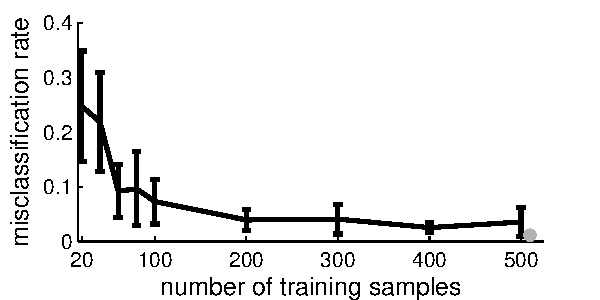
\includegraphics[width=1.0\linewidth]{../figs/hetero_easy_n10_MC5000_QAP_vs_n.pdf}
% 	\caption{Inexact graph matching can be used to approximate a consistent shuffled graph classifier.  Data in this simulation was sampled from the independent edge model described above.  For each number of training samples, we tested using 5000 test samples, and repeated 10 times.  The gray dot indicates Bayes optimal performance. (NOTE TO CEP: actually, i forgot to QAP the test data to each training class in this example.  i think it would converge much ``faster'' if i included that step. that is, faster in $s$, but now testing requires performing 2 QAPs, whereas before, it did not, so it might actually take longer.  we will see soon, as i'm running that now.)}
% 	\label{fig:1}
% \end{figure}
% 
% section simulated_experiment (end)

\subsection{Shuffled Connectome Classification} % (fold)
\label{sub:connectome_classification}

% Emboldened by the simulated performance of our unlabeled graph classifier, we decided to try it on a real-world application.  
A ``connectome'' is a brain-graph in which vertices correspond to (groups of) neurons, and edges correspond to connections between them.  Diffusion Magnetic Resonance (MR) Imaging and related technologies are making the acquisition of MR connectomes routine \cite{Hagmann2010}.  49 subjects from the Baltimore Longitudinal Study on Aging comprise this data, with acquisition and connectome inference details as reported in \cite{Gray11}.  Each connectome yields a $70$ vertex simple graph (binary, symmetric, and hollow adjacency matrix).  Associated with each graph is class label based on the sex of the individual (24 males, 25 females).  Because the vertices are labeled, we can compare the results of having the labels and not having the labels.  

Figure \ref{fig:1} reifies the above theoretical results in a particular finite sample regime.  We apply the five algorithms discussed above to sub-samples of the connectome data, which shows approximate convergence rates for this data.  Fortunately, this real data example supports the main theorems of this work.  Specifically, the $k_s$NN classifier using $\delta$ on the \emph{labeled} graphs (dashed gray line) achieves the lowest misclassification rate for all $s$, which one would expect if labels contain appropriate class signal.  Moreover, as suggested by 
Theorem \ref{thm:knninadmiss},
the $k_s$NN classifier using the inexact graph-matching Frobenius norm on the shuffled adjacency matrices, $\mt{\delta}$, performs best of all classifiers using only shuffled graphs (compare dashed black line with solid black and gray lines).  On the other hand, while the $k_s$NN classifier using the Frobenius norm on shuffled graphs, $\delta'$, must eventually converge to $L_s'$, its convergence rate is quite slow, so the classifier using standard invariants $\psi$ outperforms the simple $\delta'$ based $k_s$NN.


% The performance of a $1$NN algorithm is reported in Table \ref{tab:connectome}. When using the vertex labels, a ``labeled-$1$NN'' achieves $37\%$ misclassification rate.  Chance performance (only using the estimated prior) on this data is $49\%$.  These two numbers provide bounds on performance.  We then pass all the graphs through a shuffle channel, and implement GM-$1$NN using the approximately graph-matched Frobenius norm.  This approach yields $41\%$ misclassification rate, slightly worse than the labeled graph case.  Finally, we compare the performance of our graph-matched $1$NN algorithm with a more ``standard'' graph-invariant based algorithm, referred to as $\phi(G)$-$1$NN.  
% 
%  This results in $43\%$ misclassification rate, slightly worse than the performance of our graph-matched $1$NN.  



% The performance of the independent edge model based Bayes plugin classifier for unlabeled graphs is similarly unimpressive.  We therefore develop a hybrid approach in which the independent edge model is assumed, and parameters are estimated using the vertex labels.  Given these estimates, we can use the QAP algorithm to match each test graph to the two likelihood matrices, and then use the Bayes plugin classifier.  This approach yields a $31\%$ misclassification rate. In contrast, a ``standard'' graph invariant based approach, which computes the graph invariants from \cite{PCP10}, and plugs them into various machine learning algorithms (including the winner \cite{Crammer2008}), yields misclassification rates as low as $25\%$. 


% 
% \begin{itemize}
% 	\item \textbf{Graph Classifier} A Bayes plugin graph classifier as described in \cite{VP11a}; that is, using the labels.
% 	\item \textbf{1-QAP} Estimate the parameters using training data \emph{with} vertex labels.  Then, shuffle the test graph, \qap it to each $\mh{\PP}_y$ matrix.  The  estimated the class is $\mh{y}=\argmax_{y \in \mc{Y}}QAP(G,\mh{\PP}_y)$.   
% 	\item \textbf{48-QAP} Permuting the vertex labels, then implement \texttt{$1$NN$\circ$\qapa}.
% 	% \item \textbf{AVG-QAP}  Permuting the vertex labels, \qapa each of the 48 training graphs to the test graph.  Then, given those permuted adjacency matrices, compute the average, and then implement a standard $1$NN classifier.
% 	\item \textbf{1NN-GI} Use the graph invariant approach as described above. We provide the normalized graph invariants as inputs into a number of standard classifiers, including $k_s$NN, linear classifiers, support vector machines, random forests, and CW. On this data, the CW classifier performed best; we therefore only report its results.
% \end{itemize}
% 

\begin{figure}[htbp]
	\centering
		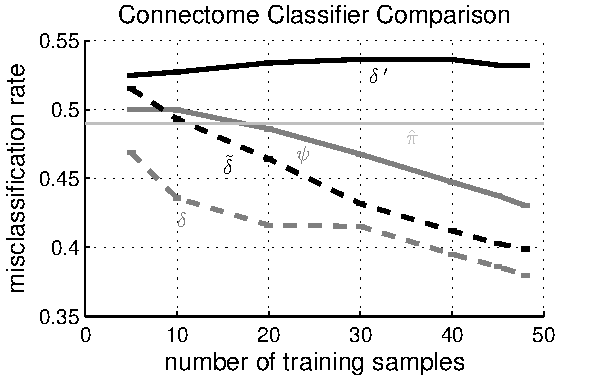
\includegraphics[width=1.0\linewidth]{../figs/Lhat_vs_s_binary.pdf}
		\caption{Connectome misclassification rates for various classifiers.  2000 Monte Carlo sub-samples of the data were performed for each $s$, such that errorbars were neglibly small.  Five classifiers were compared, as described in main text.  Note that when $s$ is larger than $20$, as predicted by theory, we have $\mh{L}^{\mh{\pi}}_s > \mh{L}^\psi_s > \mh{L}^{\mt{\delta}}_s > \mh{L}_s^\delta$. Moreover, $\mh{L}^{\delta'}_s > \mh{L}^{\mt{\delta}}_s > \mh{L}_s^\delta$.}
	\label{fig:1}
\end{figure}

% \begin{table}[h!]
% \caption{MR connectome leave-one-out misclassification rates for various $1$NN classifiers. Labeled-$1$NN refers to the $1$NN classifier using . GM-$k_s$NN refers to the approximately graph-matched Frobenius norm $k_s$NN on the shuffled graphs.  $\phi(G)$-$1$NN refers to using the Euclidean norm distance $k_s$NN on the four graph-invariants described in the main text. Chance is the Bayes plugin classifier using only the prior probabilities.  }
% \begin{center}
% \begin{tabular}{|c|c|c|c|c|}
% \hline
% Labeled-$1$NN & Shuffled-$1$NN & GM-$1$NN & $\phi(G)$-$1$NN & Chance\\
% \hline
% $37\%$ & $52\%$ & $41\%$ & $43\%$ & $49\%$ \\
%     \hline
% \end{tabular}
% \end{center}
% \label{tab:connectome}
% \end{table}%


\section{Discussion}

In this work, we address both the theoretical and practical limitations of classifying shuffled graphs, relative to labeled and unlabeled graphs.  Specifically, first we construct the notion of shuffled graphs and shuffled graph classifiers in a parallel fashion with labeled and unlabeled graphs/classifiers, as we were unable to find such notions in the literature.  Then, we show that shuffling the vertex labels results in an irretrievable situation, with a possible degradation of classification performance (Theorem \ref{thm:1}). Even if the vertex labels contained class-conditional signal, Bayes performance may remain unchanged (Theorem \ref{thm:2}).  Moreover, although one cannot hope to recover the vertex labels, one can obtain a Bayes optimal classifier by solving a large number of graph isomorphism problems (Theorem \ref{thm:3}).  This resolves a theoretical conundrum: is there a set of graph invariants that can yield a universally consistent graph classifier?  When the generative distribution is unavailable, one can induce a consistent and efficient ``unshuffling'' classifier by using a graph-matching strategy (Corollary \ref{cor:Un_Plug}).  While this unshuffling approach dominates the more na\"ive approach (Theorem \ref{thm:tdomp}), it is intractable in practice due to the difficulty of graph matching and the large number of isomorphism sets.  Instead, a Frobenius norm $k_s$NN classifier applied to the adjacency matrices may be used, which is also universally consistent (Corollary \ref{cor:Sh_knn}).  Convergence rates may be considerably sped up by using a graph-matching Frobenius norm (Theorem \ref{thm:knninadmiss}).  Surprisingly, none of the considered classifiers dominate the other for labeled data (Theorem \ref{thm:nodom}), yet asymptotically, we can order shuffled graph classifiers (Theorem \ref{thm:order}).

Because graph-matching is $\mc{NP}$-hard, we instead use an approximate graph-matching algorithm in practice (see \cite{VP11_QAP} for details).  Applying these $k_s$NN classifiers to a problem of considerable scientific interest---classifying human MR connectomes---we find that even with a relatively small sample size ($s \geq 20$), the approximately graph-matched $k_s$NN algorithm performs nearly as well as the $k_s$NN algorithm \emph{using} vertex labels, and slightly better than a $k_s$NN algorithm applied to a set of graph invariants proposed previously \cite{PCP10}.  This suggests that the asymptotics might apply even for very small sample sizes.  Thus, this theoretical insight has led us to improved practical classification performance.  Extensions to weighted or (certain) attributed graphs are straightforward.

% estimating them yields an asymptotically optimal classifier.  This suggest that efforts to estimate the vertex labels may yield useful classification results, outperforming ``standard'' graph-invariant based classifiers.  Via simulation we show that an approximate graph matching algorithm converges to the optimal performance with only about 500 training samples for a particular independent edge random graph model.   Finally, we demonstrate with connectome data that estimating the vertex labels can be useful, but that there remains room to grow to exceed misclassification performance of a carefully chosen graph invariant $\circ$ machine learning based approach on this data.   These connectome data, much like other collections of graphs, can also be equipped with both vertex and edge attributes.  As such, we hope to extend the results herein to consider the more general cases.








% use section* for acknowledgement
\ifCLASSOPTIONcompsoc
  % The Computer Society usually uses the plural form
  \section*{Acknowledgments}
\else
  % regular IEEE prefers the singular form
  \section*{Acknowledgment}
\fi

% This work was partially supported by the Research Program in Applied Neuroscience. 

% Can use something like this to put references on a page
% by themselves when using endfloat and the captionsoff option.
\ifCLASSOPTIONcaptionsoff
  \newpage
\fi


\bibliography{/Users/jovo/Research/latex/library}
\bibliographystyle{IEEEtran}

\begin{IEEEbiography}{Joshua T. Vogelstein}
 is a spritely young man, engorphed in a novel post-buddhist metaphor.

\end{IEEEbiography}


% insert where needed to balance the two columns on the last page with
% biographies
%\newpage


\begin{IEEEbiography}{Carey E. Priebe}
Buddha in training.
\end{IEEEbiography}

% Can be used to pull up biographies so that the bottom of the last one
% is flush with the other column.
% \enlargethispage{-5in}

\end{document}



